%-------------------------------------------------
%
% Part_1.tex
%
%------------------------------------------------
\chapter{Prima parte}
\label{pt1}
L'azienda produce, attraverso un macchinario automatizzato, pannelli forati. Viene richiesto di calcolare il percorso migliore che la testina possa effettuare su ogni singola piastra, al fine di massimizzare il numero di pannelli prodotti nell'unità di tempo desiderata.

%-------------------------------------------------
%
% Problem.tex
%
%------------------------------------------------
\section[Il problema]{il problema}
\label{pt1:problem}
Il problema posto ha molto in comune con il classico problema del commesso viaggiatore (\english{Travelling Salesman Problem} TSP). Si può assumere che i fori da effettuare sulla piastra siano le città da visitare, mentre i percorsi che congiungono i fori siano i possibili cammini. Ne risulta quindi un grafo completo in cui si vuole trovare uno dei migliori cammini \keyword{hamiltoniani}.

La problematica può essere espressa attraverso il seguente modello di programmazione lineare intera:

\begin{align}
MIN: &\sum_{i,j:(i,j) \in A} C_{i,j}x_{i,j} \\
S.T.: \nonumber \\ 
&\sum_{j:(0,j) \in A} x_{0,j} &=&\left|N\right|& \\
&\sum_{i:(i,k) \in A} x_{i,k} - \sum_{j:(k,j) \in A} x_{k,j} &=&1 &\forall k \in N \textbackslash \left\{0\right\} \\
&\sum_{j:(i,j) \in A} y_{i,j} &=&1 &\forall i \in N \\
&\sum_{i:(i,j) \in A} y_{i,j} &=&1 &\forall j \in N \\
&x_{i,j} &\le&\left|N\right|y_{i,j} &\forall (i,j) \in A\\
DOMINI: \nonumber \\ 
&x_{i,j} \in \mathbb{Z}_{+} &&& \forall (i,j) \in A\\
&y_{i,j} \in \left\{0, 1\right\} &&& \forall (i, j) \in A
\end{align}

%-------------------------------------------------
%
% Assumption.tex
%
%------------------------------------------------
\section[Assunzioni]{assunzioni}
\label{pt1:assumption}
Posso assumere senza alcuna perdita di generalità nel problema che il grafo G sia completo quindi siano presenti contemporaneamente gli archi che collegano il nodo $i$ al nodo $j$ e viceversa.

Al fine di ottenere migliori prestazioni si è deciso di omettere gli archi che collegano un nodo con se stesso in quanto non sono portatori di informazione utile al problema perciò la cardinalità finale della matrice associata al grafo risulta essere:

\begin{equation}
\left|A\right| = \frac{\left|N\right|\times\left(\left|N\right|-1\right)}{2} - \left|N\right|
\end{equation}

Si è infine assunto che i costi $c_{i,j}$ corrispondano alla distanza euclidea tra il nodo $i$ ed il nodo $j$ e che $c_{i,j}=c_{j,i} \forall (i,j)\in A$ ovvero il TSP sia simmetrico.

%-------------------------------------------------
%
% Generator.tex
%
%------------------------------------------------
\section[Generatori di dati]{generatori di dati}
\label{pt1:generator}
Al fine di ottenere una discreta quantità di dati su cui effettuare dei test si è progettato e conseguentemente implemento, in linguaggio $C++$,
un programma in grado di generare diverse tipologie di istanze.

Il programma è composto da alcuni oggetti di servizio che hanno lo scopo di rappresentare gli oggetti della realtà da studiare (\texttt{Plate} e \texttt{Hole}).

Tra le componenti più importanti troviamo quelle che consentono di generare i punti secondo una specifica strategia, ovvero le seguenti:

\begin{itemize}
\item\texttt{PlateGenerator}: classe base che fornisce la possibilità di generare delle piastre con le coordinate dei fori;
\item\texttt{RandomPlateGenerator}: fornisce l'algoritmo per la generazione di punti casuali su di una superficie di dimensioni date;
\item\texttt{ClusterPlateGenerator}: fornisce l'algoritmo per la generazione di punti suddivisi in un numero di \english{cluster} fornito dall'utente;
\item\texttt{CirclePlateGenerator}: fornisce l'algoritmo per la generazione di punti su di un percorso circolare chiuso.
\end{itemize}

L'ultima componente è quella che consente di serializzare una piastra e salvarne i dati essenziali su \english{file} di testo, è composta dalle seguenti classi:

\begin{itemize}
\item\texttt{ProblemGenerator}: classe base che fornisce le funzionalità di salvataggio dei dati su \english{file} e fornisce la possibilità di generare i dati del problema.
\item\texttt{EuclideanProblemGenerator}: fornisce l'algoritmo per il calcolo delle distanze euclidee tra i singoli fori che compongono la piastra.
\end{itemize}

Viene ora fornita la struttura dei \english{files} che compongono tale programma.

\dirtree{%
.1 generator.
.2 src.
.3 header.
.4 generator.
.5 CirclePlateGenerator.h.
.5 ClusterPlateGenerator.h.
.5 EuclideanProblemGenerator.h.
.5 PlateGenerator.h.
.5 RandomPlateGenerator.h.
.4 object.
.5 Hole.h.
.5 Plate.h.
.3 source.
.4 generator.
.5 CirclePlateGenerator.cpp.
.5 ClusterPlateGenerator.cpp.
.5 EuclideanProblemGenerator.cpp.
.5 ProblemGenerator.cpp.
.5 RandomPlateGenerator.cpp.
.4 object.
.5 Hole.cpp.
.5 Plate.cpp.
.2 main.cpp.
.2 makefile.
}

In Figura \ref{pt1:generator:imgs} sono riportati alcuni esempi di dati generati attraverso le varie tipologie di generatore implementate:

\begin{figure}
\centering
\begin{subfigure}[b]{0.45\textwidth}
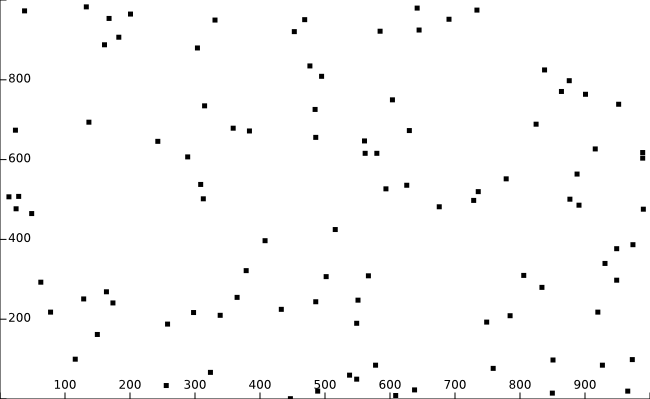
\includegraphics[width=\textwidth]{Images/Part_1/Instances/Random.png}
\caption{Random}
\label{pt1:generator:random_img}
\end{subfigure}
\quad{}
\begin{subfigure}[b]{0.45\textwidth}
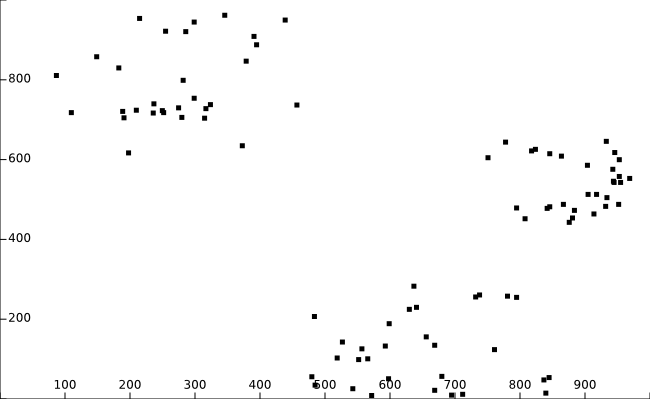
\includegraphics[width=\textwidth]{Images/Part_1/Instances/Cluster.png}
\caption{Cluster}
\label{pt1:generator:cluster_img}
\end{subfigure}

\begin{subfigure}[b]{0.5\textwidth}
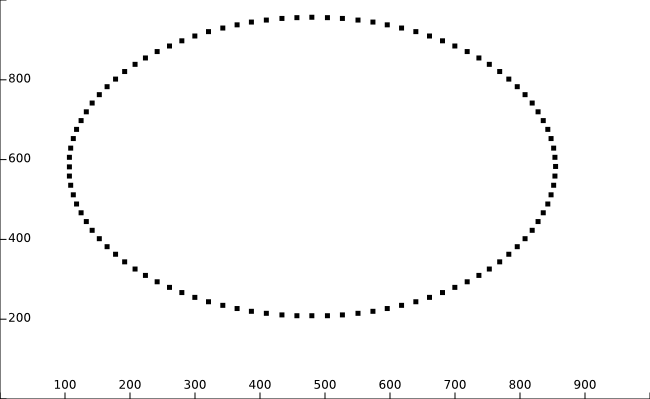
\includegraphics[width=\textwidth]{Images/Part_1/Instances/Circle.png}
\caption{Circuito}
\label{pt1:generator:Circle_img}
\end{subfigure}
\caption{Esempi di istanze generate}
\label{pt1:generator:imgs}
\end{figure}

Il programma produce due \english{files} per ogni istanza generata. Un \english{file}, con estensione \texttt{.crd}, contenente le coordinate dei punti generati ed un \english{file}, con estensione \texttt{.dat}, contenente i costi calcolati.

Per ottimizzare lo spazio di salvataggio si è deciso che, dati due nodi $i$ e $j$ nel \english{file} contenente i dati (\texttt{.dat}) viene salvato solamente il costo dell'arco $i,j$ in quanto l'arco inverso $j,i$ è deducibile dalla simmetria del grafo. Il \english{file} contiene nella prima riga il numero di fori generati e a seguire tutti i costi, uno per ogni riga.

%-------------------------------------------------
%
% Solver.tex
%
%------------------------------------------------
\section[Il risolutore]{il risolutore}
\label{pt2:solver}
Il programma con l'implementazione della meta euristica è composta dalle seguenti classi.
\newpage

\dirtree{%
.1 metaheuristic.
.2 src.
.3 header.
.4 object.
.5 Chromosome.h.
.5 Population.h.
.4 solver.
.5 GeneticAlgorithm.h.
.3 source.
.4 object.
.5 Chromosome.cpp.
.5 Population.cpp.
.4 solver.
.5 GeneticAlgorithm.cpp.
.2 main.cpp.
.2 makefile.
}

Le classi \texttt{Chromosome} e \texttt{Population} sono classi di servizio all'algoritmo e rappresentato rispettivamente un singolo cromosoma ed una popolazione.

La classe più importante è \texttt{GeneticAlgorithm} che racchiude in sé l'algoritmo illustrato in Sezione \ref{pt2:design}, ed è composta dai seguenti metodi:

\dirtree{%
.1 GeneticAlgorithm.
.2 private.
.3 readProblemDatas.
.3 getCost.
.3 getBetterChromosome.
.3 contains.
.3 fitnessFunction.
.3 initialize.
.3 crossover.
.2 public.
.3 resolve.
.3 getObjectiveValue.
}

I metodi \texttt{readProblemDatas} e \texttt{getCost} sono le medesime implementazioni che ritroviamo nel risolutore CPlex e servono a virtualizzare la matrice associata al grafo.

Il metodo \texttt{getBetterChromosome} restituisce il cromosoma con il miglior valore di \english{fitness} data una popolazione e viene utilizzato per estrarre i due \english{parent}.

Il metodo \texttt{fitnessFunction} calcola il valore di \english{fitness} dato un cromosoma.

Mentre il metodo \texttt{initialize} serve per inizializzare la popolazione iniziale prima di eseguire le evoluzioni genetiche.

Il metodo \texttt{crossover} esegue l'operazione di \english{crossover} mentre il metodo \texttt{resolve} è colui che coordina l'avanzamento delle evoluzioni.

%-------------------------------------------------
%
% Time.tex
%
%------------------------------------------------
\section[Tempi di risoluzione]{tempi di risoluzione}
\label{pt1:time}
Al fine di stabilire fino a quale dimensione il problema possa essere risolto in tempi, ragionevolmente brevi, ed in modo esatto si è deciso di valutare l'algoritmo sulle seguenti proprietà che contraddistinguono le istanze:

\begin{itemize}
\item numero di nodi del grafo;
\item distribuzione dei nodi sulla superficie della piastra.
\end{itemize}

Inizialmente si è proceduto, nel seguente modo, alla generazione delle istanze. Si sono create delle classi di istanze e per ognuna di esse si sono create 5 istanze differenti ma che condividessero le proprietà sopra riportate.

Successivamente si è eseguito l'algoritmo su ciascuna di esse e si sono registrati, nel foglio di calcolo allegato, i vari tempi di esecuzione ed il valore della funzione obiettivo.

\begin{table}[htbp]
\centering
\label{pt1:time:tabular_random}
\begin{tabular}{|c|c|c|c|}
\hline
\multicolumn{3}{|c|}{Random}\\
\hline
\textbf{Classe} & \textbf{Media (ms))} & \textbf{Media (hh:mm:ss:mmm)}\\
\hline
5   &     19 & 00:00:00:019\\
\hline
10  &     73 & 00:00:00:073\\
\hline
15  &    238 & 00:00:00:238\\
\hline
20  &    397 & 00:00:00:397\\
\hline
30  &   1872 & 00:00:01:872\\
\hline
40  &   6054 & 00:00:06:054\\
\hline
50  &  13308 & 00:00:13:308\\
\hline
60  &  20883 & 00:00:20:883\\
\hline
70  &  40550 & 00:00:40:550\\
\hline
80  &  92111 & 00:01:32:111\\
\hline
90  & 256191 & 00:04:16:191\\
\hline
100 & 506619 & 00:08:26:619\\
\hline
\end{tabular}
\caption{Tempi medi di esecuzione classe random}
\end{table}

Nella Tabella 1.1 - 1.2 - 1.3 sono riportate le medie dei tempi di esecuzione misurati.

\begin{table}[htbp]
\centering
\label{pt1:time:tabular_cluster}
\begin{tabular}{|c|c|c|c|}
\hline
\multicolumn{3}{|c|}{Cluster}\\
\hline
\textbf{Classe} & \textbf{Media (ms))} & \textbf{Media (hh:mm:ss:mmm)}\\
\hline
5   &     18 & 00:00:00:018\\
\hline
10  &     88 & 00:00:00:088\\
\hline
15  &    192 & 00:00:00:192\\
\hline
20  &    381 & 00:00:00:381\\
\hline
30  &  12685 & 00:00:12:685\\
\hline
40  &  33123 & 00:00:33:123\\
\hline
50  &   7834 & 00:00:07:834\\
\hline
60  &  35698 & 00:00:35:698\\
\hline
70  &  63743 & 00:01:03:743\\
\hline
80  & 292809 & 00:04:52:809\\
\hline
90  & 197488 & 00:03:17:488\\
\hline
100 & 823554 & 00:13:43:554\\
\hline
\end{tabular}
\caption{Tempi medi di esecuzione classe cluster}
\end{table}

\begin{table}[htbp]
\centering
\label{pt1:time:tabular_circle}
\begin{tabular}{|c|c|c|c|}
\hline
\multicolumn{3}{|c|}{Circle}\\
\hline
\textbf{Classe} & \textbf{Media (ms))} & \textbf{Media (hh:mm:ss:mmm)}\\
\hline
5   &     13 & 00:00:00:013\\
\hline
10  &     38 & 00:00:00:038\\
\hline
15  &     50 & 00:00:00:050\\
\hline
20  &     67 & 00:00:00:067\\
\hline
30  &    113 & 00:00:00:113\\
\hline
40  &    275 & 00:00:00:275\\
\hline
50  &   2754 & 00:00:02:754\\
\hline
60  &   3587 & 00:00:03:587\\
\hline
70  &   7668 & 00:00:07:668\\
\hline
80  &   3121 & 00:00:03:121\\
\hline
90  &   2415 & 00:00:02:415\\
\hline
100 &   5242 & 00:00:05:242\\
\hline
\end{tabular}
\caption{Tempi medi di esecuzione classe circle}
\end{table}

\begin{figure}
\centering
\begin{subfigure}[b]{0.9\textwidth}
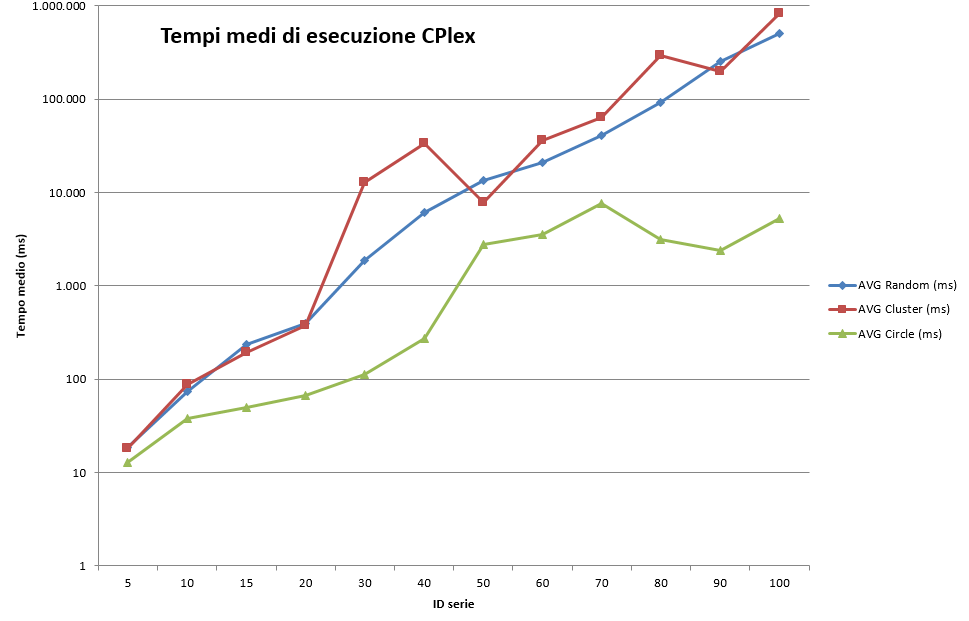
\includegraphics[width=\textwidth]{Images/Part_1/graphics/Times01.png}
\caption{Tempi di risoluzione al variare dei punti}
\label{pt1:time:time01}
\end{subfigure}

\begin{subfigure}[b]{0.9\textwidth}
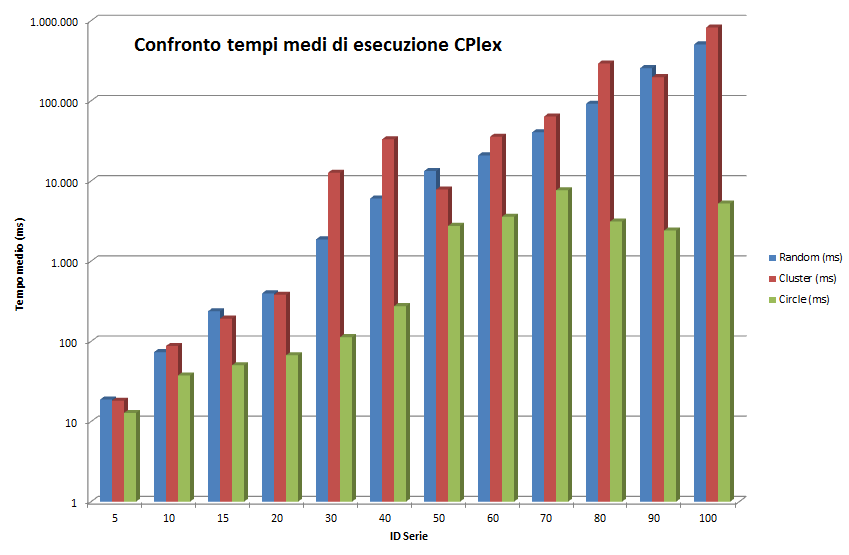
\includegraphics[width=\textwidth]{Images/Part_1/graphics/Times02.png}
\caption{Tempi di esecuzione per tipologia}
\label{pt1:time:time02}
\end{subfigure}
\caption{Confronto tempistiche}
\label{pt1:time:times}
\end{figure}

\subsection[Conclusioni]{conclusioni}
\label{pt1:time:conclusion}
Dalle misurazioni effettuate si evince che all'aumentare dei punti che compongono l'istanza vi è un significativo aumento nei tempi di risoluzione, in modo esatto, del modello.

Più precisamente, come si può notare in Figura \ref{pt1:time:time01} (attenzione alla scala dei tempi logaritmica), il tempo di risoluzione del problema cresce esponenzialmente all'aumentare dei nodi che compongono il grafo.

Essendo il TSP un problema \english{NP-hard}, la sua risoluzione esatta richiede degli algoritmi a complessità esponenziale perciò i risultati ottenuti sono coerenti con quanto atteso.

Dal grafico in Figura \ref{pt1:time:time02} è possibile osservare come anche la disposizione dei punti che compongono il grafo influisce sui tempi di risoluzione, in modo esatto, del problema. Sono da preferirsi grafi con forme geometriche ben definite al fine di poter coprire un maggior numero di punti nella stessa unità temporale.